\documentclass[conference,onecolumn]{IEEEtran}
\IEEEoverridecommandlockouts
\usepackage{cite}
\usepackage{amsmath,amssymb,amsfonts}
\usepackage{algorithmic}
\usepackage{graphicx}
\usepackage{listings}
\usepackage{float}
\usepackage{textcomp}
\usepackage{gensymb}
\usepackage{xcolor}
\usepackage[spanish]{babel}
\def\BibTeX{{\rm B\kern-.05em{\sc i\kern-.025em b}\kern-.08em
    T\kern-.1667em\lower.7ex\hbox{E}\kern-.125emX}}


\usepackage{listings}
\usepackage{xcolor}
\lstset{
  basicstyle=\ttfamily\footnotesize,
  keywordstyle=\color{blue},
  commentstyle=\color{gray},
  stringstyle=\color{red},
  frame=single,
  breaklines=true,
  numbers=left,
  numberstyle=\tiny\color{gray}
}


\begin{document}

\title{Práctica 7: Implementación de un codificador y decodificador de canal del estándar LTE}

\author{\IEEEauthorblockN{Tyrone Miguel Novillo Bravo}
\IEEEauthorblockA{\textit{Facultad de Ingenier\'ia} \\
\textit{Departamento de Telecomunicaciones}\\
Universidad de Cuenca \\
tyrone.novillo@ucuenca.edu.ec}
\and
\IEEEauthorblockN{Freddy Eduardo L\'opez Padilla}
\IEEEauthorblockA{\textit{Facultad de Ingenier\'ia} \\
\textit{Departamento de Telecomunicaciones}\\
Universidad de Cuenca\\
freddy.lopez@ucuenca.edu.ec}
}

\maketitle

\begin{abstract}
En esta práctica se implementan en Python los dos códigos correctores de errores especificados
por el estándar LTE: el código convolucional \textit{tail-biting} de tasa $1/3$, decodificado con el
algoritmo de Viterbi de decisión suave, y el turbo código de tasa $1/3$, formado por dos
codificadores convolucionales recursivos sistemáticos concatenados en paralelo mediante un
entrelazador QPP y decodificado de forma iterativa con dos decodificadores APP (BCJR).
Ambos códigos se integran en una cadena OFDM sobre un canal multitrayecto Pedestrian~A con ruido
AWGN, y se evalúan transmitiendo texto y una imagen de prueba (Lena). Los resultados muestran la
ganancia de codificación de ambos esquemas frente a la transmisión sin codificar: a
7~dB con 16-QAM el turbo código recupera el texto sin errores
(BER $=$ 0.000) mientras que sin codificación la BER es de 0.090.
Como contraparte, se cuantifica el costo computacional: la decodificación turbo es en promedio
4.2$\times$ más lenta que la de Viterbi, evidenciando el compromiso entre capacidad de
corrección y tiempo de procesamiento.
\end{abstract}

\begin{IEEEkeywords}
LTE, codificación de canal, códigos convolucionales, turbo códigos, Viterbi, BCJR, QPP, BER, OFDM.
\end{IEEEkeywords}

\IEEEpeerreviewmaketitle


\section*{Objetivos}
\begin{itemize}
    \item Implementar el codificador y el decodificador del código convolucional \textit{tail-biting}
          de tasa $1/3$ especificado en el estándar LTE.
    \item Implementar el codificador y el decodificador del turbo código de tasa $1/3$ de LTE
          (dos codificadores RSC de 8 estados con entrelazador interno QPP).
    \item Integrar ambos códigos en una cadena de transmisión OFDM sobre un canal multitrayecto
          Pedestrian~A y verificar su funcionamiento transmitiendo texto e imágenes.
    \item Comparar el desempeño de ambos códigos frente a la transmisión sin codificar mediante
          curvas de BER frente a SNR obtenidas por simulación de Monte Carlo.
    \item Medir y comparar el tiempo de ejecución de ambos esquemas de codificación y
          decodificación, y analizar el compromiso entre ganancia de codificación y costo
          computacional.
\end{itemize}


\section{Introducción}

Los sistemas de comunicaciones inalámbricas operan sobre canales hostiles en los que el
desvanecimiento multitrayecto y el ruido introducen errores en los bits transmitidos. Para
prevenir y corregir estos errores, la capa física incorpora una etapa de \emph{codificación de
canal} que agrega redundancia controlada a la información: cada bit de datos se esparce en varios
bits de código, de manera que el receptor pueda recuperar la información original incluso cuando
parte de los bits llega corrompida \cite{dahlman2014}. El estándar LTE adopta dos códigos con este
fin: un código convolucional \textit{tail-biting} para los canales de control y un turbo código
---piedra angular de su esquema de codificación--- para los canales de datos \cite{ts36212}.

En esta práctica se implementan desde cero, en Python, el codificador y el decodificador de ambos
códigos, siguiendo las especificaciones del estándar y el material del curso \cite{vazquez2024}.
Los códigos se integran en la cadena OFDM desarrollada en las prácticas anteriores (canal
Pedestrian~A \cite{itu1225} con ruido AWGN) y se evalúan de tres maneras: transmitiendo un texto de
prueba (\textit{lorem ipsum}), transmitiendo la imagen Lena, y mediante simulaciones de Monte
Carlo que producen curvas de BER frente a SNR. Adicionalmente, se mide el tiempo de ejecución de
cada esquema para cuantificar el costo computacional de la decodificación iterativa del turbo
código frente a la decodificación de Viterbi del código convolucional.

\section{Marco teórico}

\subsection{Códigos convolucionales y decodificación de Viterbi}

Un codificador convolucional es un sistema con memoria construido con registros de desplazamiento
y sumadores módulo 2: cada bit de entrada produce $n$ bits de salida que dependen del bit actual y
de los $m$ bits anteriores, con tasa de código $1/n$ \cite{vazquez2024}. LTE emplea un código de
tasa $1/3$ con $m=6$ memorias (64 estados) y polinomios generadores $G_0=133_8$, $G_1=171_8$ y
$G_2=165_8$. En lugar de agregar bits de cola, el estándar usa la técnica
\textit{tail-biting}: el registro se inicializa con los últimos 6 bits del bloque, de modo que el
estado inicial y el final coinciden y no se desperdicia ancho de banda \cite{ts36212}. Al ser una
máquina de estados finita, el código queda descrito por un diagrama de \textit{trellis}, y la
decodificación consiste en hallar la secuencia más probable que lo recorre; el algoritmo de
Viterbi \cite{viterbi1967} resuelve esta búsqueda de forma óptima y eficiente.

\subsection{Turbo códigos y decodificación iterativa}

Los turbo códigos \cite{berrou1993} pertenecen a la categoría de codificación convolucional
concatenada en paralelo (PCCC): dos codificadores convolucionales recursivos sistemáticos (RSC)
idénticos, de 8 estados en LTE, procesan el mismo bloque de $K$ bits, el primero en orden natural
y el segundo tras un entrelazador interno. La salida son tres flujos: los bits sistemáticos
$S_k$, la paridad $P1_k$ del primer RSC y la paridad $P2_k$ del segundo, lo que da una tasa
ligeramente menor que $1/3$ por los bits de terminación de \textit{trellis}
\cite{vazquez2024}. El entrelazador de LTE es la permutación polinomial cuadrática (QPP)
$\pi(i)=(f_1 i+f_2 i^2)\bmod K$, con coeficientes tabulados para 188 tamaños de bloque entre 40 y
6144 bits \cite{ts36212}. La decodificación es \emph{iterativa}: dos decodificadores APP
(\textit{a posteriori probability}, algoritmo BCJR \cite{bcjr1974}) se pasan mutuamente decisiones
suaves ---información extrínseca--- a través del entrelazador, y con cada iteración la estimación
mejora, alcanzando un rendimiento cercano al límite de Shannon a costa de una complejidad
computacional proporcional al número de iteraciones \cite{dahlman2014}.


\section{Metodología -- Desarrollo de la práctica}
% ============================================================

La implementación se realizó en Python con NumPy, reutilizando la cadena OFDM de las prácticas
anteriores (modulación QAM, IFFT + prefijo cíclico, canal Pedestrian~A, ecualización ZF). La
Fig.~\ref{fig:diagramas} resume la estructura de los dos codificadores implementados.

\begin{figure}[H]
    \centering
    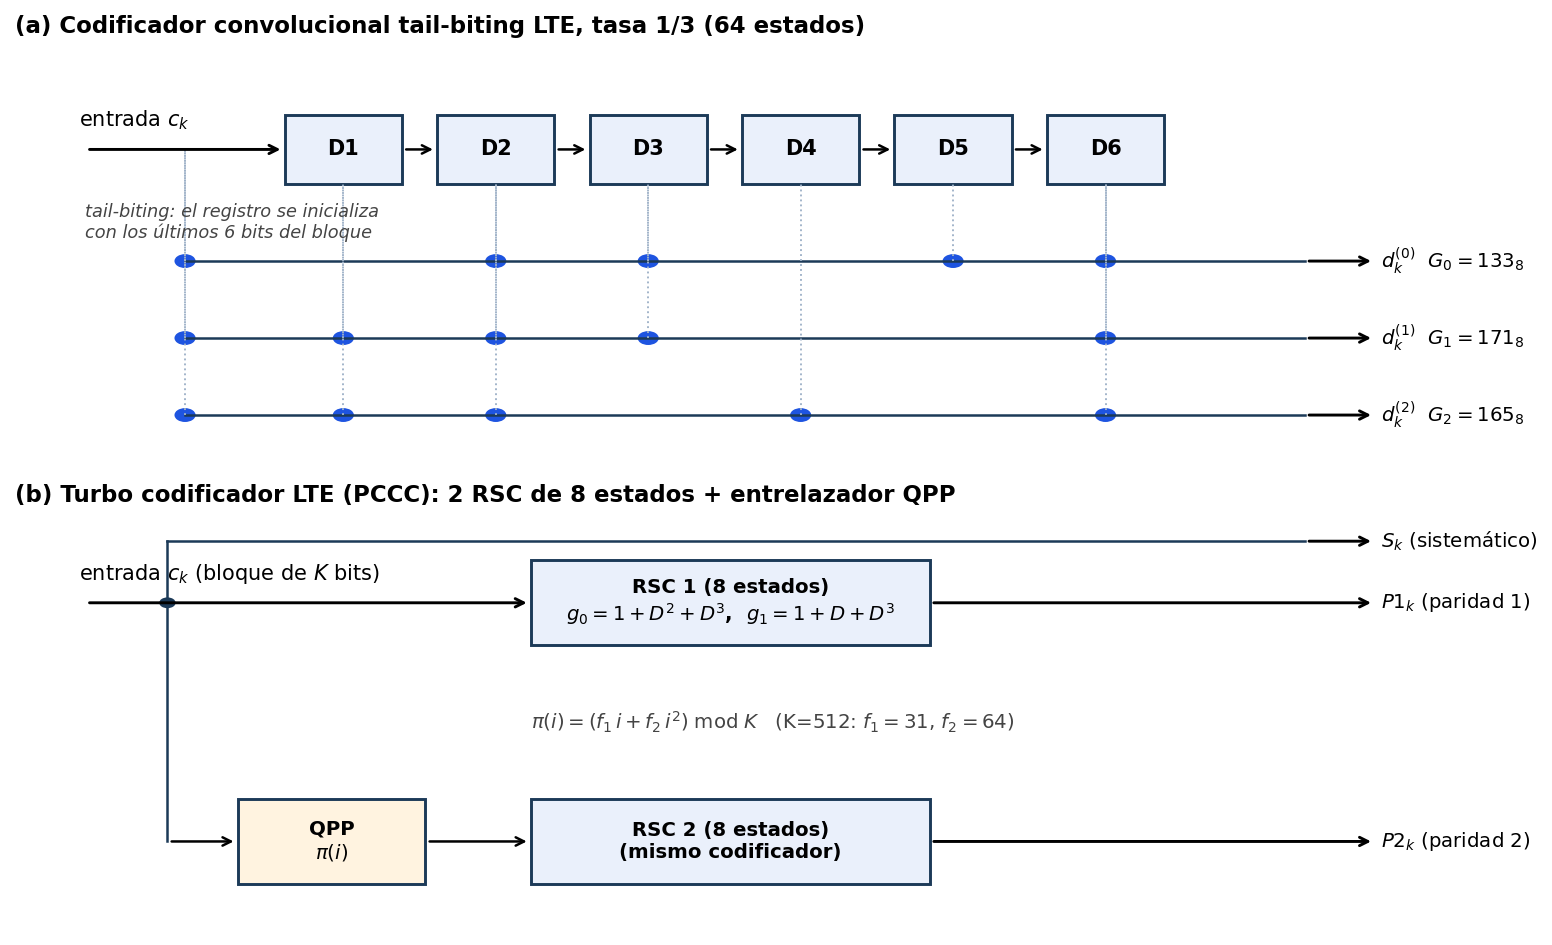
\includegraphics[width=0.95\textwidth]{img/diagrama_codificadores.png}
    \caption{Esquema de los codificadores implementados: (a) convolucional \textit{tail-biting}
    de tasa 1/3 con sus tres polinomios generadores; (b) turbo codificador PCCC con dos RSC de
    8 estados y entrelazador QPP.}
    \label{fig:diagramas}
\end{figure}

\subsection{Generación del código convolucional tail-biting}

El codificador se implementó como una máquina de estados de 6 memorias. Cada generador octal se
expande en 7 \textit{taps} (entrada y memorias $D_1$--$D_6$) y la salida de cada rama es la suma
módulo 2 de los bits seleccionados por sus \textit{taps}. La propiedad \textit{tail-biting} se
obtiene inicializando el registro con los últimos 6 bits del bloque, lo que garantiza que el
estado final iguale al inicial sin transmitir bits de cola:

\begin{lstlisting}[language=Python]
G_CONV = (0o133, 0o171, 0o165)      # polinomios generadores (octal)

def codificar_convolucional(bits):
    K = len(bits)
    taps = _conv_taps()             # 7 taps por generador: [entrada, D1..D6]
    # tail-biting: el registro arranca con los ULTIMOS 6 bits del bloque
    estado = sum(int(bits[K - 1 - i]) << i for i in range(6))
    d = np.empty((K, 3), dtype=np.uint8)
    for k in range(K):
        estado, d[k] = _conv_paso(estado, int(bits[k]), taps)
    return d.reshape(-1)            # 3 bits de codigo por bit de entrada
\end{lstlisting}

donde \texttt{\_conv\_paso} calcula las tres salidas como XOR de los \textit{taps} activos y
desplaza el registro ($D_1 \leftarrow$ entrada, $D_{i+1} \leftarrow D_i$).

\subsection{Generación del turbo código}

El elemento base es el codificador RSC de 8 estados, definido por la realimentación
$g_0(D)=1+D^2+D^3$ y la paridad $g_1(D)=1+D+D^3$. Su \textit{trellis} se tabula recorriendo los
8 estados y las 2 entradas posibles:

\begin{lstlisting}[language=Python]
def _rsc_trellis():
    # g0 = 1 + D^2 + D^3 (realimentacion),  g1 = 1 + D + D^3 (paridad)
    for s in range(8):
        m1, m2, m3 = s & 1, (s >> 1) & 1, (s >> 2) & 1
        for u in range(2):
            a  = u ^ m2 ^ m3                 # realimentacion
            z  = a ^ m1 ^ m3                 # bit de paridad
            ns = a | (m1 << 1) | (m2 << 2)   # estado siguiente
\end{lstlisting}

El entrelazador QPP es una sola línea vectorizada; para el tamaño de bloque adoptado en la
práctica, $K=512$, el estándar define $f_1=31$ y $f_2=64$:

\begin{lstlisting}[language=Python]
def qpp_interleaver(K):
    f1, f2 = QPP[K]                  # K=512 -> (f1, f2) = (31, 64)
    i = np.arange(K)
    return (f1 * i + f2 * i * i) % K
\end{lstlisting}

El turbo codificador aplica el mismo RSC dos veces ---al bloque en orden natural y al bloque
entrelazado--- y cada RSC se termina de forma independiente con 3 bits de cola que fuerzan el
registro al estado cero, por lo que cada flujo tiene longitud $K+4$ como indica el estándar:

\begin{lstlisting}[language=Python]
def codificar_turbo(bits):
    K = len(bits)
    perm = qpp_interleaver(K)
    z1, t1s, t1p = _rsc_codificar(bits, trellis)         # paridad 1
    z2, t2s, t2p = _rsc_codificar(bits[perm], trellis)   # paridad 2
    # salida: sistematico + paridad 1 + paridad 2 + colas  (tasa ~ 1/3)
    return {"sys": bits, "par1": z1, "par2": z2, ...}
\end{lstlisting}

\subsection{Recepción: demapeo suave y decodificadores}

Tras la ecualización ZF, el demapeo no decide bits (decisión dura) sino que calcula un LLR
(logaritmo de la razón de verosimilitud) por bit, ponderado por la calidad
$|H[k]|^2$ de la subportadora que lo transportó: los bits que cayeron en un desvanecimiento
entran al decodificador con poca confianza y los demás los corrigen. Este intercambio de
decisiones suaves es el que habilita la ganancia de codificación \cite{vazquez2024}.

El código convolucional se decodifica con Viterbi de decisión suave sobre el \textit{trellis} de
64 estados; como el \textit{tail-biting} no fija el estado inicial ni el final, se recorre el
bloque circular varias vueltas (4 en esta implementación) y se decodifica la última. El turbo
código se decodifica con dos decodificadores APP (BCJR en su versión max-log) en lazo de
realimentación durante 6 iteraciones:

\begin{lstlisting}[language=Python]
def decodificar_turbo(Lsys, Lp1, Lp2, ..., perm, K, n_iter=6):
    La1 = np.zeros(K)                       # informacion a priori inicial
    for _ in range(n_iter):
        Le1 = _bcjr_maxlog(Lsys, Lp1, La1, ...)              # APP 1
        Le2 = _bcjr_maxlog(Lsys[perm], Lp2, Le1[perm], ...)  # APP 2
        La1 = Le2[invperm]                  # extrinseca de vuelta al APP 1
    L_total = Lsys + Le1 + La1              # canal + ambos extrinsecos
    return (L_total < 0).astype(np.uint8)   # decision final por signo
\end{lstlisting}

\subsection{Escenario de simulación y medición de tiempos}

La información se segmenta en bloques de $K=512$ bits que se codifican, se modulan (QPSK o
16-QAM), se transmiten por la cadena OFDM y se decodifican por lotes. La Tabla~\ref{tab:params}
resume los parámetros. Como fuentes de datos se usaron el texto \textit{lorem ipsum} de dos
párrafos (8\,208 bits) y la imagen Lena reescalada a $96\times96$ píxeles RGB
(221\,184 bits, 432 bloques). El tiempo de procesamiento de cada transmisión
(codificación + OFDM + canal + decodificación) se midió con \texttt{time.perf\_counter()}, y las
curvas de BER y de tiempo frente a SNR se obtuvieron por Monte Carlo con 3 corridas
independientes por punto e intervalos de confianza del 95\,\% (t de Student).

\begin{table}[H]
\centering
\caption{Parámetros de la simulación.}
\label{tab:params}
\begin{tabular}{|l|l|}
\hline
\textbf{Parámetro} & \textbf{Valor} \\
\hline
Ancho de banda / $\Delta f$ / CP & 5 MHz / 15 kHz / normal (4.7 $\mu$s) \\
Subportadoras útiles / $N_{FFT}$ & 300 / 512 \\
Canal & Pedestrian A (ITU-R M.1225), Rayleigh por \textit{tap} + AWGN \\
Ecualización / demapeo & Zero-Forcing / LLR max-log ponderado por $|H|^2$ \\
Modulaciones & QPSK, 16-QAM \\
Tamaño de bloque $K$ & 512 bits (QPP: $f_1=31$, $f_2=64$) \\
Código convolucional & tasa 1/3, $G=(133,171,165)_8$, \textit{tail-biting}, Viterbi suave (4 vueltas) \\
Turbo código & tasa 1/3, 2 RSC de 8 estados, BCJR max-log, 6 iteraciones \\
Monte Carlo & SNR de 0 a 15 dB, 3 corridas por punto, IC 95\,\% \\
\hline
\end{tabular}
\end{table}


\section{Evaluación -- Análisis de resultados}

\subsection{Transmisión de texto (lorem ipsum)}

El texto de prueba se transmitió a 7~dB con 16-QAM usando los tres esquemas sobre
realizaciones equivalentes del canal. Sin codificación el texto llega ilegible en varios tramos;
el convolucional reduce los errores a cerca de la tercera parte y el turbo código lo recupera
exactamente:

\begin{lstlisting}
--- Original -------------------------------------------------------
Lorem ipsum dolor sit amet, consectetur adipiscing elit. Donec sodales ipsum vel ante vulputate, id feugiat ligula imperdiet. [...]

--- Sin codificar (BER = 0.090, 5 ms) ----------
?orem`ipsqo dodmb ri4 amet,$c/.sectet?r ad)?m3ci/g ehmt. Dnnecaso?!me3 )`sum r?l aotg wuh?u?at?$ i?$fauwh`t$lkg=,$`iip-Vtie4o ?mks$l1cq?!?uBpi6,`P2u??um n/n mdbtls Sed,0asctmsan |?nci$ent n)si. Y~ hac0hebmte?Qe`platea d}ct?ms`n ?t [...]

--- Convolucional (BER = 0.030, 95 ms) --------
Lorem ipsum dolor sit amet, consectetur adipiscing elit. Don>?[??dales ipsum vel ante vulputate, id feugiat ligula imperdic????8is??cup??2rpis, pretium non lectus sed, accumsan tincidunt nisi. In hac habitasse platea dictumst. Ut  [...]

--- Turbo (BER = 0.000, 176 ms) --------------
Lorem ipsum dolor sit amet, consectetur adipiscing elit. Donec sodales ipsum vel ante vulputate, id feugiat ligula imperdiet. Duis lacus turpis, pretium non lectus sed, accumsan tincidunt nisi. In hac habitasse platea dictumst. Ut [...]
\end{lstlisting}

Este resultado ilustra el propósito de la codificación de canal: con la misma energía por símbolo
y el mismo canal, la redundancia de tasa $1/3$ más la decisión suave convierten una transmisión
inutilizable en una transmisión sin errores.

\subsection{Transmisión de imagen (Lena)}

La Fig.~\ref{fig:lena} repite el experimento con la imagen Lena ($96\times96$ RGB,
432 bloques de código) a 7~dB con 16-QAM. Sin codificación la imagen se
recibe cubierta de ruido de sal y pimienta (BER $\approx$ $8.6\times10^{-2}$); el código
convolucional reduce la BER en un factor de ${\sim}6$ y el turbo código en un factor de
${\sim}27$, entregando la imagen prácticamente intacta.

\begin{figure}[H]
    \centering
    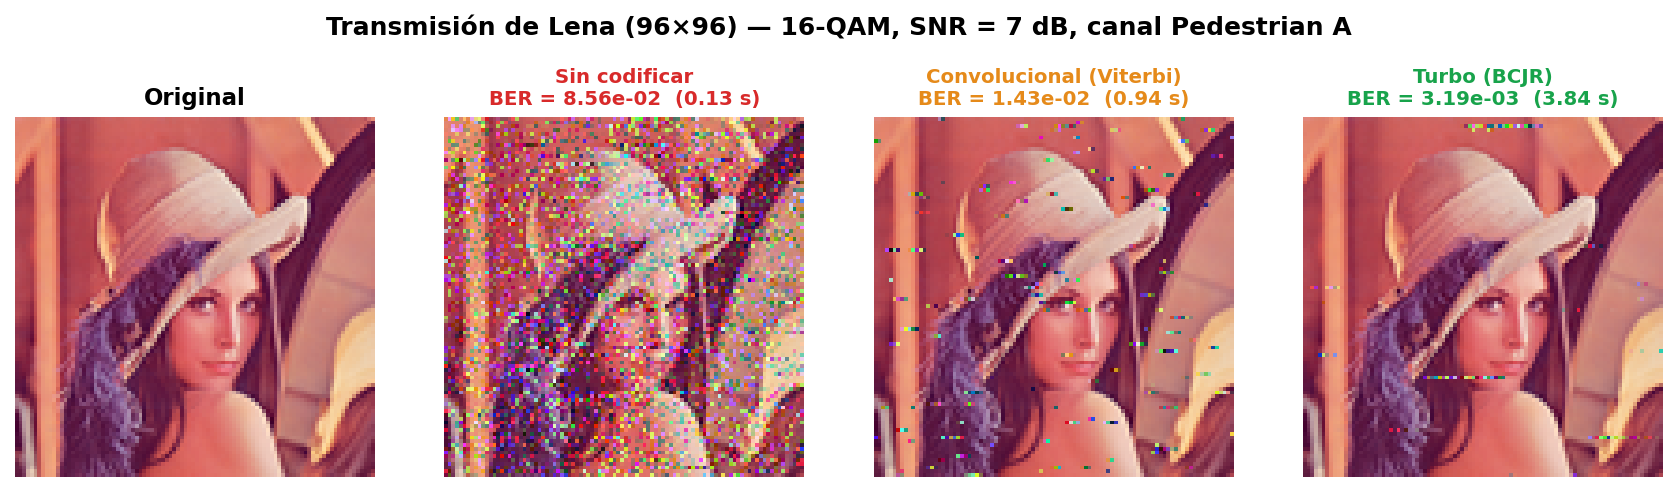
\includegraphics[width=0.98\textwidth]{img/lena_codificacion.png}
    \caption{Recuperación de la imagen Lena con cada esquema de codificación
    (16-QAM, SNR = 7 dB, canal Pedestrian A). Bajo cada imagen se indica la BER y el
    tiempo de procesamiento de la transmisión.}
    \label{fig:lena}
\end{figure}

\subsection{BER frente a SNR}

La Fig.~\ref{fig:ber} muestra las curvas de BER frente a SNR obtenidas por Monte Carlo
transmitiendo la imagen Lena completa en cada corrida (221\,184 bits por corrida,
3 corridas por punto). Se observa el orden esperado
turbo $\leq$ convolucional $\leq$ sin codificar en todo el barrido y para ambas modulaciones:

\begin{itemize}
    \item El código convolucional aporta una ganancia de codificación sostenida: a 8~dB con
          16-QAM reduce la BER de $6.7\times10^{-2}$ a $9.9\times10^{-3}$.
    \item El turbo código exhibe el ``acantilado'' característico de la decodificación iterativa:
          con QPSK cae por debajo de $10^{-5}$ desde los 4~dB, y con 16-QAM se desploma entre 4 y
          8~dB (de $2.7\times10^{-2}$ a $5.0\times10^{-4}$), alcanzando el piso de la simulación
          en 12~dB. Por debajo de ese umbral el intercambio iterativo de información extrínseca
          pierde su ventaja e incluso puede amplificar los errores (a 0~dB con 16-QAM su BER
          supera a la de la transmisión sin codificar), comportamiento típico de esta familia de
          códigos.
    \item Sin codificación la BER decae lentamente con la SNR, dominada por los desvanecimientos
          profundos del canal Pedestrian~A: aún a 15 dB persisten errores.
\end{itemize}

\begin{figure}[H]
    \centering
    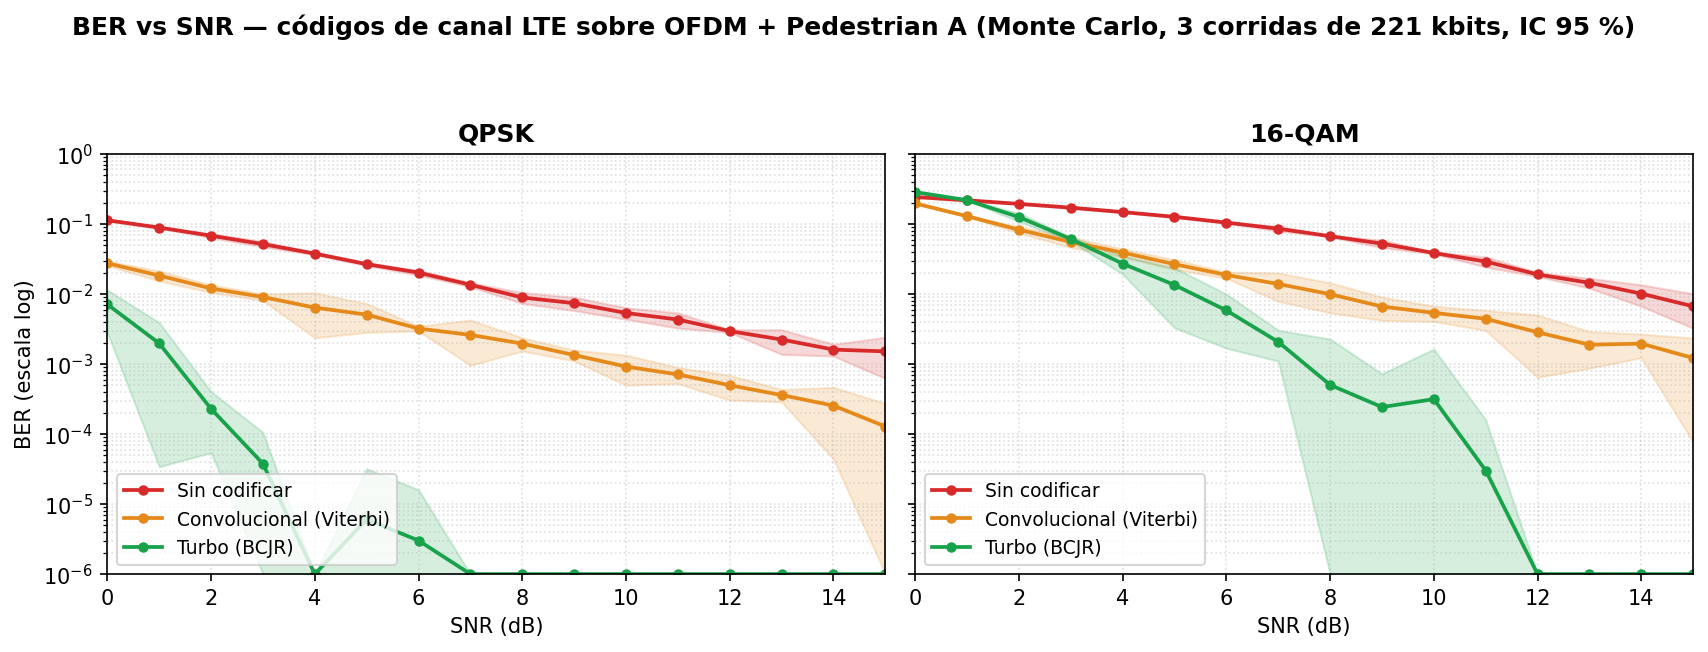
\includegraphics[width=0.98\textwidth]{img/ber_snr.png}
    \caption{BER frente a SNR para los tres esquemas, con QPSK (izquierda) y 16-QAM (derecha).
    Sombreado: intervalo de confianza del 95\,\%.}
    \label{fig:ber}
\end{figure}

\subsection{Tiempo de ejecución frente a SNR}

La Fig.~\ref{fig:tiempo} presenta el tiempo de procesamiento de la transmisión completa en
función de la SNR, y la Tabla~\ref{tab:tiempos} resume los promedios. Se destacan tres
observaciones:

\begin{itemize}
    \item El tiempo es esencialmente \emph{independiente de la SNR} en los tres esquemas: tanto
          Viterbi como BCJR realizan la misma cantidad de operaciones sin importar cuán ruidosa
          llegue la señal (en esta implementación el número de iteraciones turbo es fijo).
    \item El turbo código es el más costoso: en promedio 3.84~s por transmisión con
          16-QAM (8.9~ms por bloque de 512 bits), unas 4.2 veces el tiempo
          del convolucional (0.99~s). La diferencia proviene del decodificador: BCJR se
          ejecuta dos veces por iteración durante 6 iteraciones (12 pasadas por el
          \textit{trellis}), mientras que Viterbi hace una única pasada.
    \item La transmisión sin codificar es la más rápida (0.14~s) pero, como muestran las
          Figs.~\ref{fig:lena} y \ref{fig:ber}, a costa de una BER inaceptable en este canal.
\end{itemize}

\begin{figure}[H]
    \centering
    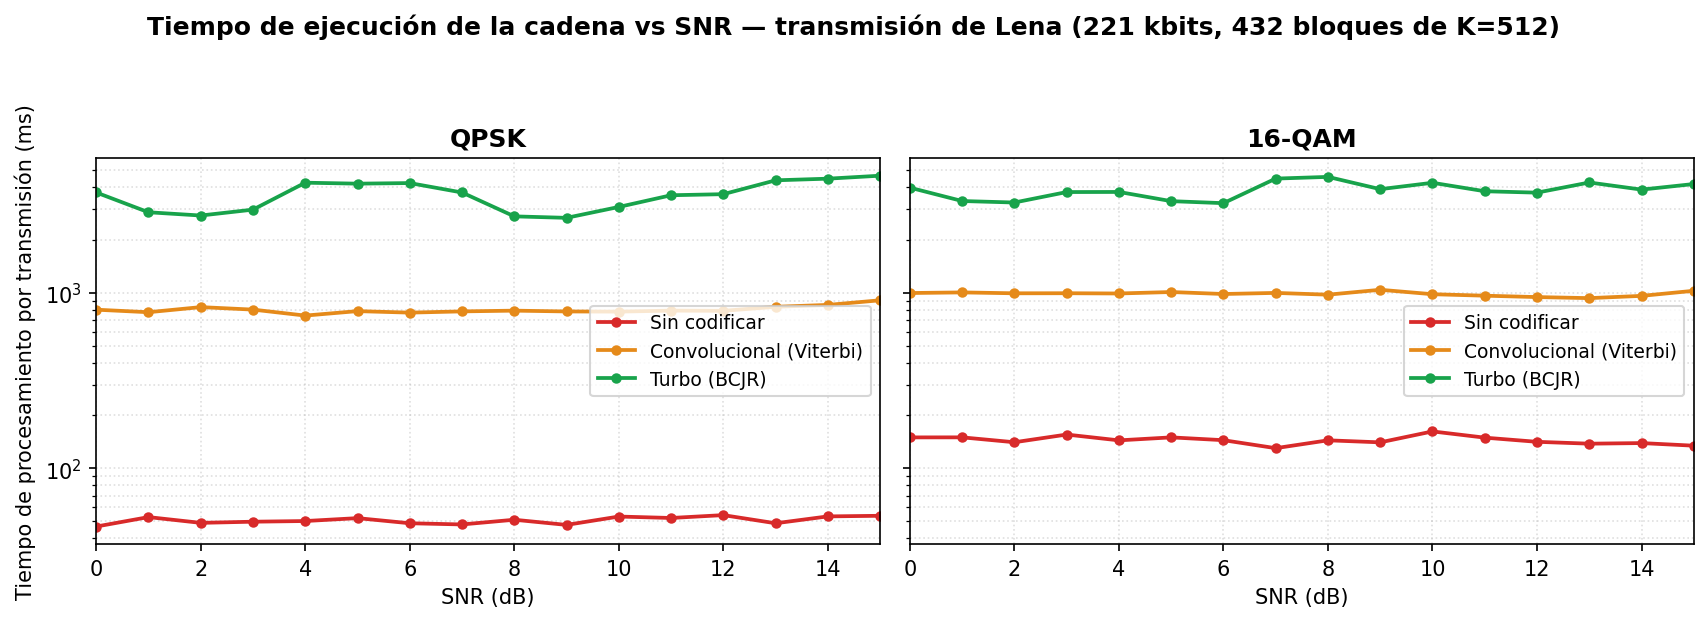
\includegraphics[width=0.98\textwidth]{img/tiempo_snr.png}
    \caption{Tiempo de procesamiento por transmisión frente a SNR (escala logarítmica), con QPSK
    (izquierda) y 16-QAM (derecha).}
    \label{fig:tiempo}
\end{figure}

\begin{table}[H]
\centering
\caption{Resumen del compromiso BER--tiempo (promedios sobre el barrido de SNR, transmisión de
432 bloques).}
\label{tab:tiempos}
\begin{tabular}{|l|c|c|c|c|c|c|}
\hline
 & \multicolumn{3}{c|}{\textbf{QPSK}} & \multicolumn{3}{c|}{\textbf{16-QAM}} \\
\hline
\textbf{Esquema} & BER @ 4 dB & BER @ 8 dB & Tiempo (s) & BER @ 4 dB & BER @ 8 dB & Tiempo (s) \\
\hline
Sin codificar   & $3.8\times10^{-2}$  & $8.9\times10^{-3}$  & 0.05  & $1.5\times10^{-1}$  & $6.7\times10^{-2}$  & 0.14 \\
Convolucional   & $6.4\times10^{-3}$ & $2.0\times10^{-3}$ & 0.80 & $3.9\times10^{-2}$ & $9.9\times10^{-3}$ & 0.99 \\
Turbo           & $\le 10^{-6}$ & $\le 10^{-6}$ & 3.61 & $2.7\times10^{-2}$ & $5.0\times10^{-4}$ & 3.84 \\
\hline
\end{tabular}
\end{table}

El compromiso queda entonces cuantificado: el turbo código compra su rendimiento
casi-Shannon con un decodificador $\sim$4.2$\times$ más lento que Viterbi. Esto es
consistente con el reparto de tareas del estándar: LTE reserva el turbo código para los canales
de datos, donde el volumen de información justifica el costo, y usa el convolucional en los
canales de control, cortos y sensibles a la latencia \cite{dahlman2014}.

% ============================================================
\section{Conclusiones}

Se implementaron y verificaron el codificador y el decodificador de los dos códigos de canal del
estándar LTE. El código convolucional \textit{tail-biting} de tasa $1/3$ quedó definido por sus
tres polinomios generadores $(133,171,165)_8$ y su decodificación con Viterbi de decisión suave;
el turbo código, por la concatenación en paralelo de dos RSC de 8 estados separados por el
entrelazador QPP y su decodificación APP iterativa. La transmisión de texto y de la imagen Lena
demostró de forma tangible la ganancia de codificación: en condiciones donde la transmisión sin
codificar resulta inutilizable (BER $\sim10^{-1}$--$10^{-2}$), el convolucional reduce la BER
típicamente entre 3 y 7 veces y el turbo código recupera la información prácticamente sin errores.

Las curvas de Monte Carlo confirmaron el orden turbo $\leq$ convolucional $\leq$ sin codificar en
todo el barrido de SNR y para ambas modulaciones, con el ``acantilado'' característico del turbo
código: por encima de un umbral de pocos dB la BER se desploma al piso de la simulación
($\le 10^{-6}$), comportamiento que explica su elección como piedra angular de la codificación de
datos en LTE.

La medición de tiempos cuantificó el precio de ese rendimiento: la decodificación turbo
(2 pasadas BCJR $\times$ 6 iteraciones) resultó $\sim$4.2$\times$ más lenta que la
decodificación de Viterbi, y ambas son independientes de la SNR. Este compromiso
rendimiento--complejidad se refleja directamente en el diseño del estándar, que asigna el turbo
código a los canales de datos y el convolucional a los canales de control. Como trabajo futuro se
podría incorporar el \textit{rate matching} del estándar (perforado y versiones de redundancia
HARQ) y una parada temprana de las iteraciones turbo, que reduciría el tiempo medio de
decodificación en los puntos de SNR alta.


% ============================================================
\bibliographystyle{IEEEtran}
\bibliography{referencias}


\end{document}
